\documentclass[12pt]{beamer}
\usepackage{../latex-sty/mypres}
\usepackage[utf8]{inputenc}
\usepackage[T2A]{fontenc}
\usepackage[russian]{babel}

\usefonttheme[onlymath]{serif}

\expandafter\def\expandafter\insertshorttitle\expandafter{%
  \insertshorttitle\hfill%
  \insertframenumber\,/\,\inserttotalframenumber}
\title[Семинар 11]{Методы оптимизации. \\
 Семинар 11. Двойственность.}
\author{Александр Катруца}
\institute{Московский физико-технический институт\\
Факультет Управления и Прикладной Математики} 
\date{\today}

\begin{document}
\begin{frame}
\maketitle
\end{frame}

\begin{frame}{Напоминание}
\begin{itemize}
\item Существование решения оптимизационной задачи 
\item Условия оптимальности для
\begin{itemize}
\item общей задачи оптимизации
\item задачи безусловной оптимизации
\item задачи оптимизации с ограничениями типа равенств
\item задачи оптимизации с ограничениями типа равенств и неравенств
\end{itemize}
\end{itemize}
\end{frame}

\begin{frame}{Обозначения}
\small
\begin{block}{Задача}
\vspace{-5mm}
\begin{equation*}
\begin{split}
& \min\limits f(x) = p^*\\
\text{s.t. } & g_i(x) = 0, \; i = 1,\ldots,m\\
& h_j(x) \leq 0, \; j = 1,\ldots, p
\end{split}
\end{equation*}
\end{block}

\begin{block}{Лагранжиан}
\vspace{-2mm}
\begin{equation*}
L(x, \blambda, \bmu) = f(x) + \sum\limits_{i=1}^m\lambda_i g_i(x) + \sum\limits_{j=1}^p \mu_j h_j(x)
\vspace{-2mm}
\end{equation*}
\end{block}

\begin{block}{Двойственные переменные}
Вектора $\bmu$ и $\blambda$ называются двойственными переменными.
\end{block}

\begin{block}{Двойственная функция}
Функция $g(\bmu, \blambda) = \inf\limits_x L(x, \blambda, \bmu)$ называется двойственной функцией Лагранжа.
\end{block}

\end{frame}

\begin{frame}{Свойства двойственной функции}
\small
\begin{block}{Вогнутость}
Двойственная функция является {\color{red}{вогнутой}} как инфимум аффинных функций по $(\bmu, \blambda)$ вне зависимости от того, является ли исходная задача выпуклой.
\end{block}

\begin{block}{Нижняя граница}
Для любого $\blambda$ и для $\bmu \geq 0$ выполнено $g(\bmu, \blambda) \leq p^*$.
\end{block}

\begin{block}{Двойственная задача}
\vspace{-5mm}
\begin{equation*}
\begin{split}
& \max g(\bmu, \blambda) = d^*\\
\text{s.t. } & \bmu \geq 0
\end{split}
\end{equation*}
\end{block}

\begin{block}{Зачем?}
\begin{itemize}
\vspace{-2mm}
\item Двойственная задача выпукла независимо от того, выпукла ли прямая
\vspace{-3mm}
\item Нижняя оценка \textbf{может} достигаться
\end{itemize}
\end{block}
\end{frame}

\begin{frame}{Связь с сопряжённой функцией}
Рассмотрим задачу
\begin{equation*}
\begin{split}
&\min f_0(x) \\
\text{s.t. } & \bA\bx \leq \mathbf{b}\\
& \bC\bx = \bd
\end{split}
\end{equation*}
Тогда
\begin{equation*}
\begin{split}
& g(\blambda, \bmu) = \inf_{\bx} (f_0(\bx) + \blambda^{\T}(\bA\bx - \mathbf{b}) + \bmu^{\T}(\bC\bx - \bd)) = \\
& - \mathbf{b}^{\T}\blambda - \bmu^{\T}\bd + \inf_{\bx}(f_0(\bx) + (\bA^{\T}\blambda + \bC^{\T}\bmu)^{\T}\bx) = \\
& - \mathbf{b}^{\T}\blambda - \bmu^{\T}\bd - f_0^*(-\bA^{\T}\blambda - \bC^{\T}\bmu)
\end{split}
\end{equation*}
Области определений двойственной и сопряжённой функций связаны:
\[
\text{dom } g = \{ (\blambda, \bmu) \; | \; -\bA^{\T}\blambda - \bC^{\T}\bmu \in \text{dom } f^*_0 \}
\] 
\end{frame}

\begin{frame}{Примеры}
Найти двойственную функцию:
\begin{itemize}
\item Решение СЛУ минимальной нормы 
\vspace{-3mm}
\begin{equation*}
\begin{split}
& \min \| \bx\|^2_2\\
\text{s.t. } & \bA\bx = \mathbf{b}
\end{split}
\end{equation*}
\item Линейное программирование
\vspace{-3mm}
\begin{equation*}
\begin{split}
& \min \bc^{\T}\bx\\
\text{s.t. } & \bA\bx = \mathbf{b}\\
& \bx \geq 0
\end{split}
\end{equation*}
\item Задача разбиения
\vspace{-3mm}
\begin{equation*}
\begin{split}
& \min \bx^{\T}\bW\bx\\
\text{s.t. } & x^2_i = 1, \; i = 1,\ldots,n
\end{split}
\end{equation*}
\end{itemize}
\end{frame}

\begin{frame}{Слабая и сильная двойственность}
\small
\begin{block}{Определение}
Оптимальные значения целевой функции в прямой и двойственной задаче связаны соотношением 
\vspace{-3mm}
\[
d^* \leq p^*.
\vspace{-4mm}
\]
Если $d^* < p^*$, то свойство называют слабой двойственностью.
Если $d^* = p^*$, то~--- сильной двойственностью.
\end{block}

\begin{block}{Замечание}
Слабая двойственность есть всегда по построению двойственной задачи.
\end{block}

\begin{block}{Вопросы}
\begin{itemize}
\item При каких условиях выполняется сильная двойственность?
\vspace{-7mm}
\item Как использовать двойственность для проверки оптимальности?
\end{itemize}
\end{block}
\end{frame}

\begin{frame}{Критерий субоптимальности}
По построению $p^* \geq g(\blambda, \bmu)$, поэтому $f_0(x) - p^* \leq f_0(x) - g(\blambda, \bmu) = \varepsilon$.
\begin{block}{Определение}
Разность $f_0(x) - g(\blambda, \bmu)$ называется \emph{двойственным зазором} и является оценкой сверху для разности текущего и оптимального значения функции.
\end{block}
Способы использования:
\begin{itemize}
\item критерий остановки в итерационном процессе
\item теоретическая оценка сходимости алгоритма
\item проверка оптимальности данной точки
\end{itemize}
\end{frame}

\begin{frame}{Условия Слейтера}
\begin{block}{Теорема}
Если задача выпуклая и существует $x$, лежащий внутри допустимой области, т.е. ограничения типа неравенств выполнены как строгие неравенства, то выполнено свойство сильной двойственности.
\end{block}

\begin{itemize}
\item Решение СЛАУ наименьшей нормы
\item Линейное программирование
\item Квадратичное программирование с квадратичными огранчиениями
%\item Невыпуклая задача с сильной двойственностью
\end{itemize}
\end{frame}

\begin{frame}{Геометрическая интерпретация}
\begin{center}
$\min\limits_{x} f_0(x), \text{ where } f_1(x) \leq 0.$
\end{center}
$
g(\lambda) = \inf\limits_{(u, t) \in \mathcal{G}} (t + \lambda u) \qquad \mathcal{G} = \{ (f_1(x), f_0(x)) \; | \; x \in \mathcal{D} \}
$
\vspace{-10mm}
\begin{columns}
\begin{column}{0.6\textwidth}
\begin{figure}
\centering
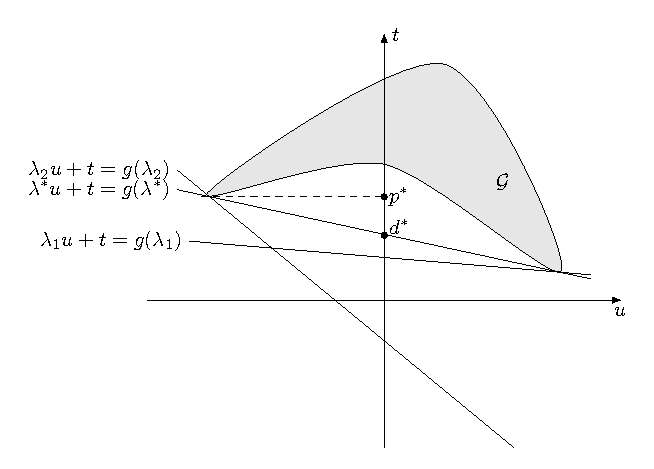
\includegraphics[scale=0.7]{duality_geom.pdf}
\end{figure}
\end{column}
~
\begin{column}{0.4\textwidth}
\begin{itemize}
\item $\lambda = 0$
\item $\lambda^*$~--- оптимальное значение
\item $\lambda > \lambda^*$
\end{itemize}
\end{column}
\end{columns}

\end{frame}

\begin{frame}{Условия дополняющей нежёсткости}
Пусть $\bx^*$ и $(\bmu^*, \blambda^*)$ решения прямой и двойственной задачи. То есть
\begin{equation*}
\begin{split}
& f(\bx^*) = g(\bmu^*, \blambda^*) = \inf\limits_{\bx} L(\bx, \blambda, \bmu) \leq \\
& f(\bx^*) + \sum\limits_{i=1}^m\lambda^*_i g_i(\bx^*) + \sum\limits_{j=1}^p \mu^*_j h_j(\bx^*) \leq\\
& f(\bx^*), \qquad \bmu \geq 0 
\end{split}
\end{equation*}

\begin{block}{Условия дополняющей нежёсткости}
\[
\mu^*_j h_j(\bx^*) = 0, \qquad j = 1,\ldots,p 
\]
Для каждого неравенства
\begin{itemize}
\item либо множитель Лагранжа равен нулю
\item либо оно активно.
\end{itemize} 
\end{block}
\end{frame}

\begin{frame}{Условия Каруша-Куна-Таккера}
Из прошлого семинара известны необходимые условия~ККТ: 
\begin{enumerate}
\item $g_i(x^*) = 0$~--- допустимость в прямой задаче
\item $h_j(x^*) \leq 0$~--- допустимость в прямой задаче
\item $ \mu^*_j \geq 0$~--- допустимость в двойственной задаче
\item $\mu^*_jh_j(x^*) = 0$~--- условие дополняющей нежёсткости
\item $\nabla_x L(x^*, \blambda^*, \bmu^*) = 0$~--- стационарность лагранжиана по прямым переменным
\end{enumerate}
Пример $(\bP \in \mathbb{S}^n_+)$
\begin{equation*}
\begin{split}
& \min\limits_{\bx \in \bbR^n} \frac{1}{2}\bx^{\T}\bP\bx + \bq^{\T}\bx + r\\
\text{s.t. } & \bA\bx = \mathbf{b}
\end{split}
\end{equation*}
\end{frame}

\begin{frame}{Механическая интерпретация}
\begin{figure}
\centering
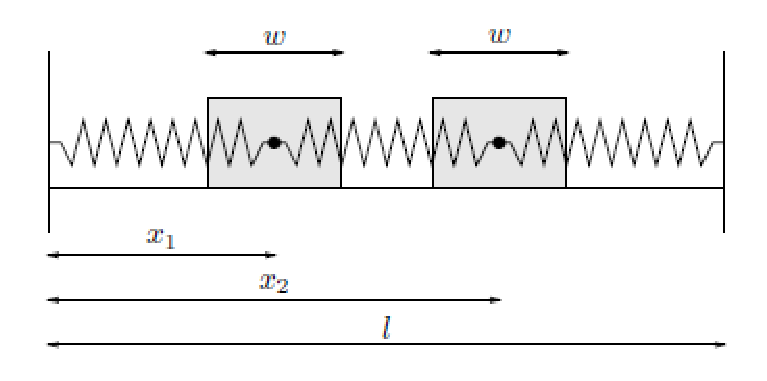
\includegraphics[scale=0.5]{kkt_mechanics.eps}
\end{figure}
Поиск устойчивого положения системы:
\begin{equation*}
\begin{split}
& \min_{\bx \in \bbR^3} \frac{1}{2}k_1x_1^2 + \frac{1}{2}k_2(x_2 - x_1)^2 + \frac{1}{2}k_3 (l - x_2)^2\\
\text{s.t. } & \frac{w}{2} - x_1 \leq 0\\
& w + x_1 - x_2 \leq 0\\
& \frac{w}{2} - l + x_2 \leq 0
\end{split}
\end{equation*}

\end{frame}

\begin{frame}{Примеры}
\footnotesize
\begin{itemize}
\item Отрицательная энтропия при линейных ограничениях
\vspace{-3mm}
\begin{equation*}
\begin{split}
& \min\limits_{\bx \in \bbR^n} \sum\limits_{i=1}^n x_i \log x_i\\
\text{s.t. } & \bA\bx \leq \mathbf{b}\\
& \mathbf{1}^{\T}\bx = 1
\end{split}
\end{equation*} 
\item Сформулировать двойственную задачу и по её решению найти решение прямой задачи:
\begin{equation*}
\begin{split}
& \min \frac{1}{2}x^2 + 2y^2 + \frac{1}{2}z^2 + x + y + 2z\\
\text{s.t. } & x+2y+z = 4
\end{split}
\end{equation*}
\item Релаксация Лагранжа для задачи бинарного линейного программирования:
\begin{equation*}
\begin{split}
&\min\limits_{\bx \in \bbR^n} \bc^{\T}\bx\\
\text{s.t. } & \bA \bx \leq \mathbf{b}\\
& x_i \in \{0,1 \}, \quad i = 1,\ldots,n
\end{split}
\end{equation*}
\end{itemize}
\end{frame}

\begin{frame}{Резюме}
\begin{itemize}
\item Двойственая задача: что это такое и зачем она нужна?
\item Сильная и слабая двойственность
\item Условия Слейтера
\item Геометрическая и механическая интерпретации
\end{itemize}
\end{frame}
\end{document}
